\documentclass[../TakeYourPill.tex]{subfiles}
\graphicspath{{\subfix{images/}}}

\begin{document}

Pro přidání úvodní obrazovky jsem použil knihovnu \textit{material-intro} \cite{intro}. Tato knihovna se postará o všechen layout a logiku úvodní obrazovky. Má jednoduché API a tak jediné, co jsem do aplikace přidal, byla aktivita \textit{AppIntroActivity} dědící ze třídy \textit{IntroActivity} a v ní přidal slidy pomocí funkce \textit{addSlide()}. Obrázky ve slidech jsem vyfotil v android emulátoru a upravil v programu \textit{GIMP}. Úvodní obrazovka se spustí pouze když uživatel aplikaci spustí poprvé. Toto je zajištěno tak, že do trvalé paměti aplikace\footnote{SharedPrefs} se po ukončení této aktivity uloží proměnná \textit{firstRun} s hodnotou \textit{false}.

\begin{figure}[h]
    \centering
    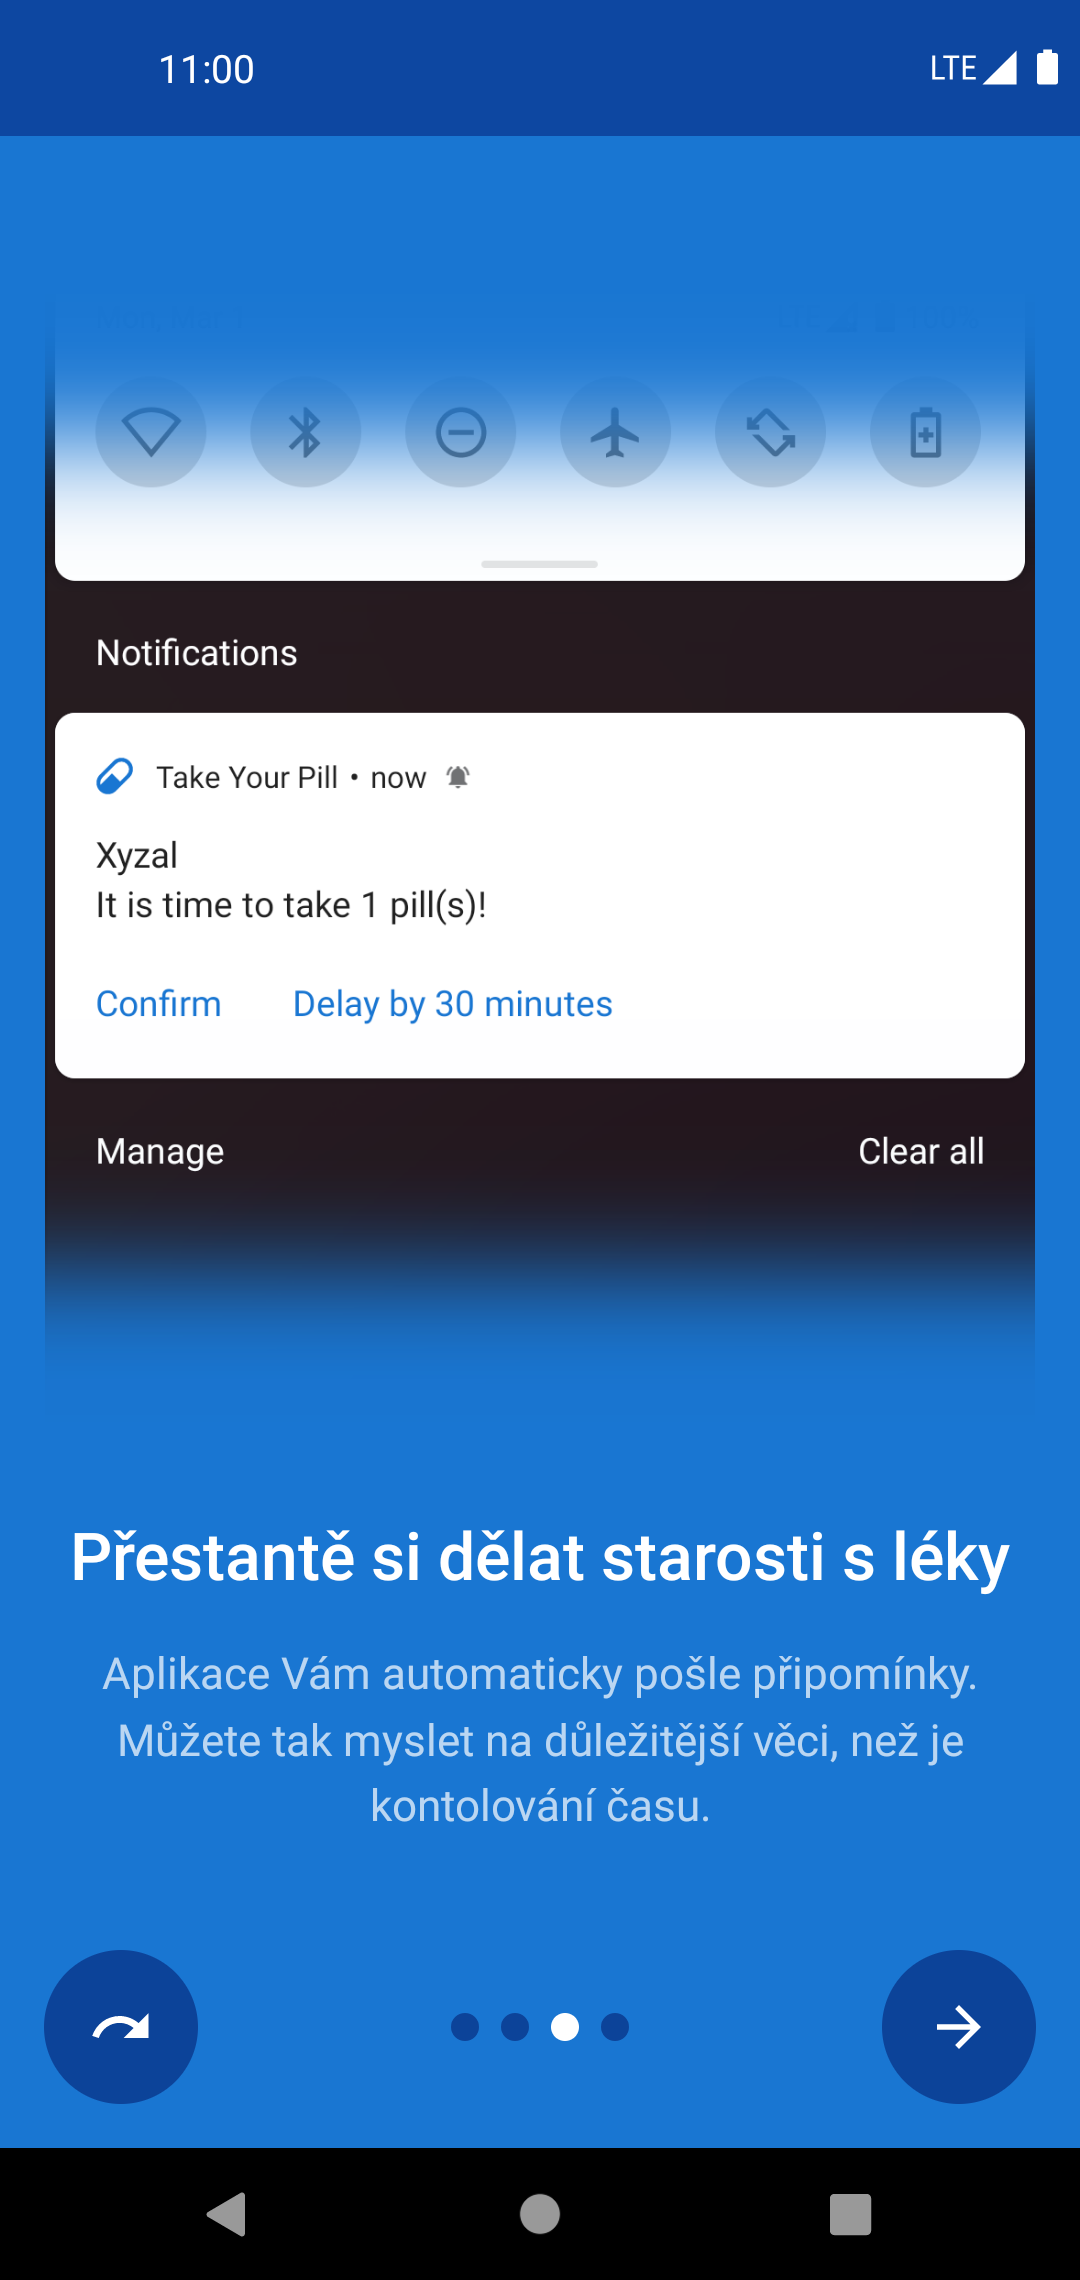
\includegraphics[width=0.25\textwidth]{app-intro-screenshot}
    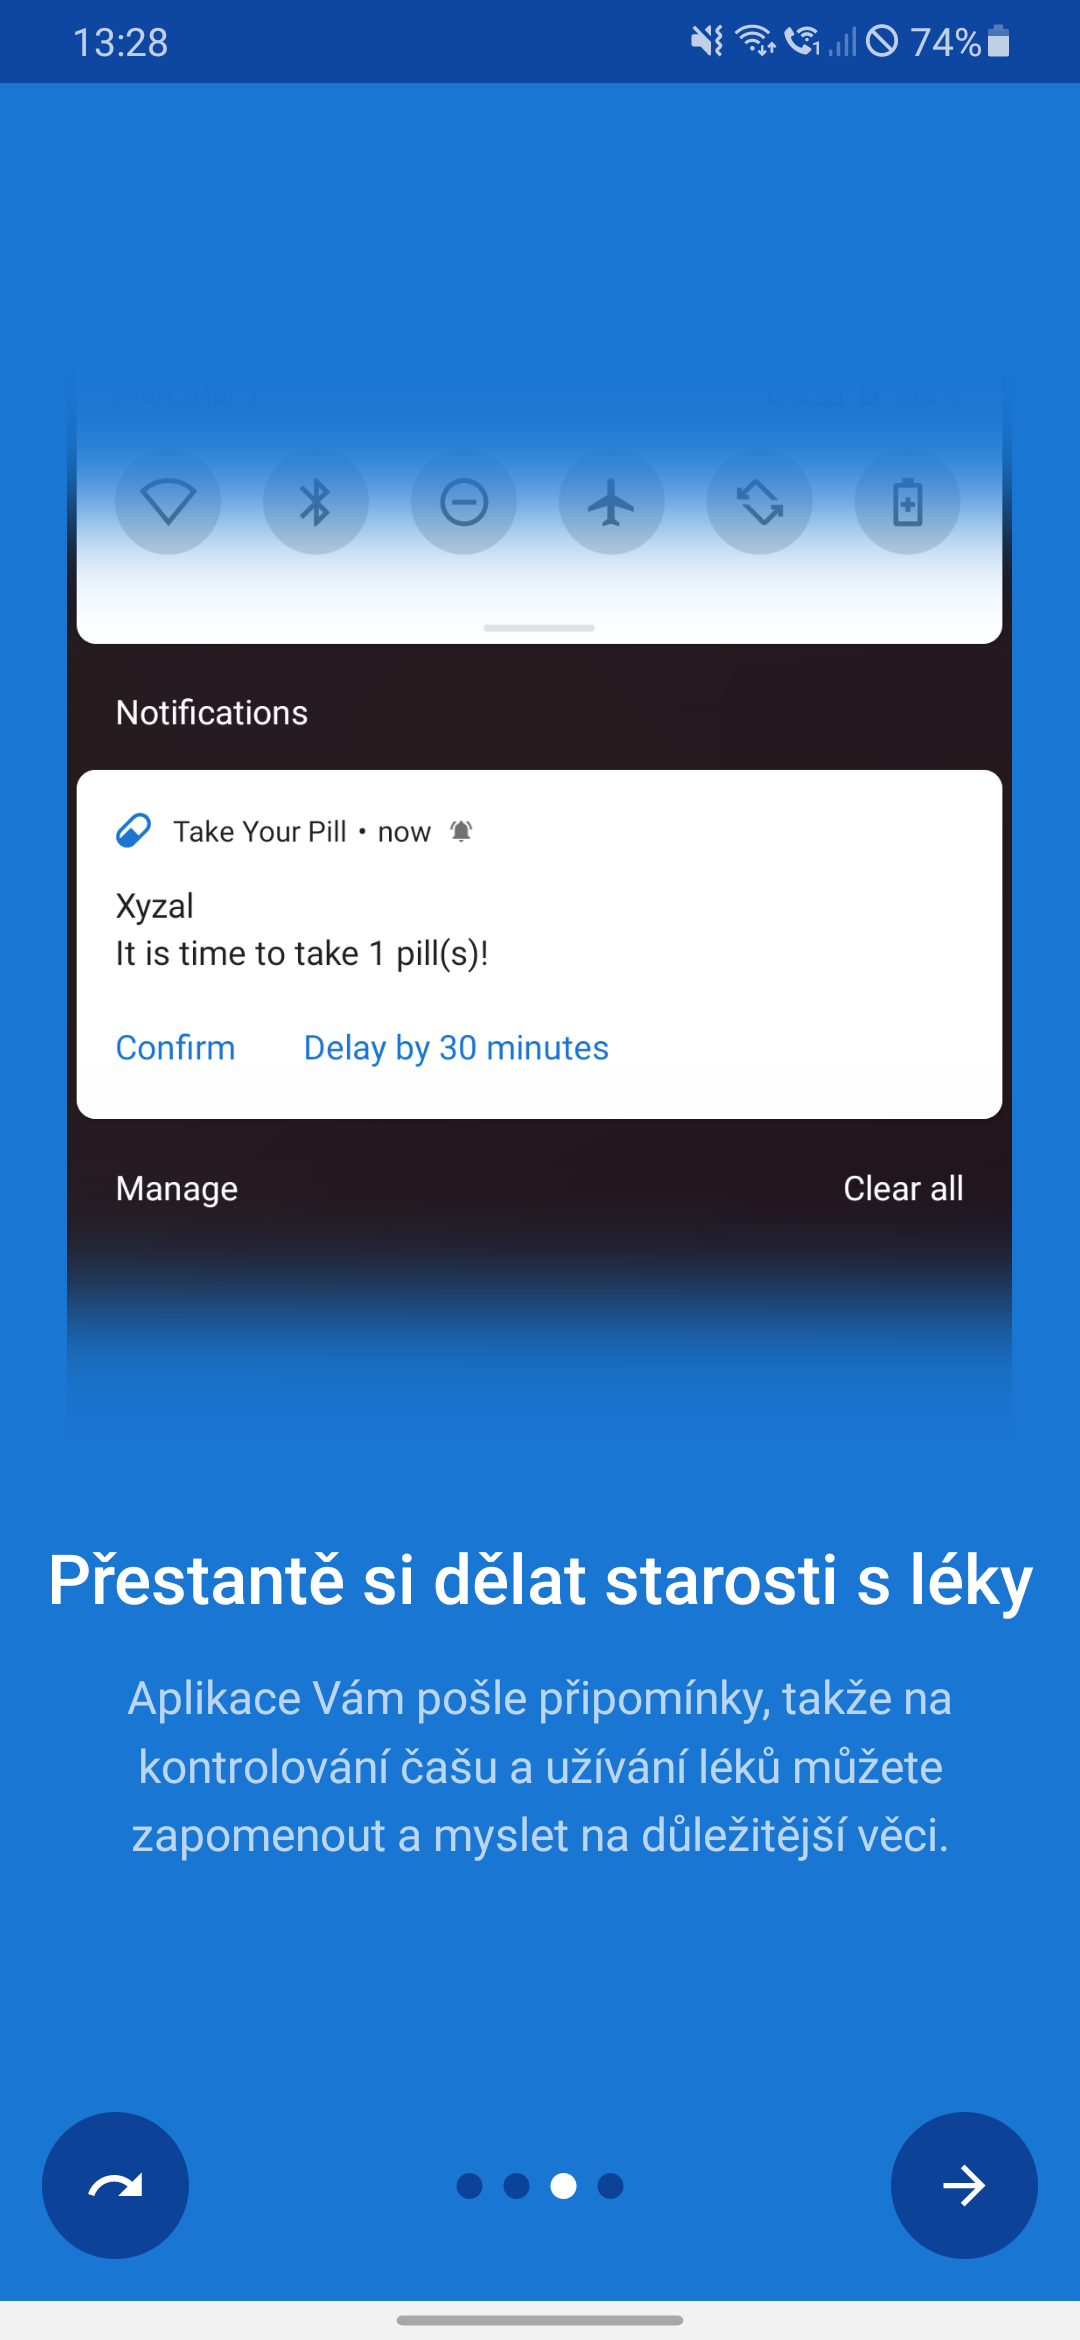
\includegraphics[width=0.25\textwidth]{app-intro-screenshot-2}
    \caption{Úvodní obrazovka}
\end{figure}

\end{document}
